Autonomous drone flight has wide-ranging applications from power line inspection to package delivery. One important aspect of autonomous drone flight that is lacking is autonomous landing, as a result of the challenges that are specific to landing in an unknown environment, such as obstacles and uneven ground. A typical method to autonomously land drones is to use computer vision and fiducial markers to identify and travel to a safe landing area.\cite{visual_servoing}\cite{high_velocity_landing}\cite{vision_based_x_platform} Fiducial markers provide a means of calculating the pose of the drone with respect to the landing pad. However these methods have not been integrated into the two main open source autonomous flight softwares: ArduPilot and PX4. These softwares offer only more primitive methods focusing on initial GPS localization and maintaining a constant rate of descent over the landing pad while performing simpler horizontal position correction based on vision. These methods are subject to GPS inaccuracies and dangers of landing even if the landing pad is not seen, meaning that the drone cannot guarantee a landing in a safe location. Other methods which have used fiducial markers typically use fixed, downward-facing cameras which can lose sight of the landing pad if the drone is not in the correct orientation, or in the final phase of landing where the drone is too close to the landing pad for the marker to be entirely in the camera's field of view.

This project provides a means of overcoming the aforementioned challenges by maintaining the drone's view of the landing pad through an automatically aimed, gimbal-mounted camera which points at the landing pad's fiducial marker throughout the entire landing, and by allowing descent only in a specific region around the landing pad. It also uses a newer fiducial marker called WhyCon \cite{whycon_paper} (shown in Figure \ref{fig:whycon}), which is more computationally efficient than the typically used April Tag \cite{apriltag_paper} (shown in Figure \ref{fig:april_tag}).

\begin{figure}
    \centering
    \begin{subfigure}[b]{0.25\textwidth}
        \centering
        
\includegraphics[width=\textwidth]{images/tag_36h11.png}
        \caption{April Tag marker.}
        \label{fig:april_tag}
    \end{subfigure}
    \begin{subfigure}[b]{0.25\textwidth}
        \centering
        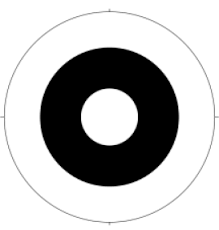
\includegraphics[width=\textwidth]{images/whycon.png}
        \caption{WhyCon marker.}
        \label{fig:whycon}
    \end{subfigure}
    \caption{Examples of fiducial markers which enable visual pose estimation.}
\end{figure}

This project involved three students: Joshua Springer and Garret Forhofer, hired as part of the RANNIS Student Innovation Fund, and Kjartan Már Andersen, hired on a summer job through Reykjavik University. The work was carried out at Reykjavik University.